% Paper II: quantum state of the frozen horizon.
% Companion to the phenomenology paper; same Springer SVJour3 class.
\documentclass[twocolumn]{svjour3}

\usepackage{amsmath,amssymb}
\usepackage{graphicx}
\usepackage{booktabs}
\usepackage[hidelinks]{hyperref}

\newcommand{\Mpl}{M_{\rm Pl}}
\newcommand{\Mpc}{\,{\rm Mpc}^{-1}}
\newcommand{\HH}{H_H}

\journalname{Eur. Phys. J. C}

\begin{document}

\title{The quantum state of the frozen horizon: Neumann contour,
classicalizing thimble, and the discrete mode-crossing kernel}
\titlerunning{The quantum state of the frozen horizon}
\author{Stilian Pandev}
\authorrunning{S. Pandev}
\institute{Independent researcher \\ \email{stilianpandev@gmail.com}}
\date{Received: date / Accepted: date}

\maketitle

\begin{abstract}
Consider a metric $f(R)$ theory with an exact constant-curvature
solution at which the scalaron is tachyonic. Such a theory possesses a
compact Euclidean four-sphere as a candidate origin for the inflationary
history, and the saddle is admissible as a decay channel when it carries
exactly one negative mode: for a tachyon of mass $m_H^2=-\mu^2H_H^2$ this
requires $0<\mu^2<4$. We show that this
condition is necessary but not sufficient. Continuing the unstable direction
through the equator and demanding that the growing Lorentzian branch be real
selects a unique complex contour, rotated by an angle $\theta(\mu^2)$; the
Born measure along it is normalizable only when $\cos2\theta<0$, which fails
below $\mu^2=7/4$. The threshold is exact and structural: at $\mu^2=7/4$ the
growth exponent is $s=1/2$, so the two Lorentzian exponents $s$ and $-(3+s)$
differ by an integer, and this is the unique degeneracy of the mode equation
interior to the one-negative-mode window. Admissible tachyonic horizons
therefore satisfy $7/4<\mu^2<4$. We develop the state of such a saddle in
detail at the unit spectral gap $\mu^2=d-1=3$: the boundary kernel is
computed mode by mode and confirms that the homogeneous direction is the sole
negative eigenvalue while all inhomogeneous scalar and physical tensor
harmonics are Gaussian suppressed; the classicalizing contour lies at
$\theta=71.216^\circ$; and the background lapse integral, performed exactly
under a Neumann regularity condition, retains both Hartle--Hawking saddles
with nonvanishing intersection numbers while eliminating the tunneling pair.
Scalar and metric perturbations decouple at quadratic order, so the joint
intersection number is unity throughout the region carrying semiclassical
probability. Because the spatial sections are $S^3$, the early noise is not a
continuum: harmonic $n$ enters the long-wavelength sector at $N_n=\ln(n+1)$
exactly and the first shell injects three times the continuum variance, so
the exit is a discrete first-passage process. In the worked example of the
companion paper the first shell maps to $k\simeq4.5\times10^{-12}\Mpc$, far
outside the present horizon, so the discreteness is a property of the initial
state and not of the observable sky. Global Stokes behaviour, the
conformal-factor contour, and a derived decoherence threshold remain open.
\keywords{Quantum cosmology \and $f(R)$ gravity \and No-boundary proposal
\and Picard--Lefschetz theory \and Inflation}
\end{abstract}

\section{Introduction}
\label{sec:intro}
A metric $f(R)$ theory whose curvature function admits a root of
$Rf_R-2f=0$ at finite curvature possesses an exact de Sitter solution. If the
scalaron is tachyonic there, with $m_H^2=-\mu^2H_H^2$, the solution is
unstable and its Euclidean continuation is a regular compact four-sphere: the
$f(R)$ counterpart of a Hawking--Moss saddle \cite{HawkingMoss1982}, and a
candidate origin for an inflationary history that begins at finite size
rather than at a singularity. Constructions of this kind have a long
lineage, from the original anomaly-supported de Sitter stage of $R^2$
inflation \cite{Starobinsky1980,Vilenkin1985} to the local polynomial
realization analyzed in the companion paper \cite{PandevI}.

A classical saddle, however, does not determine the quantum state built upon
it. The integration contour over the unstable direction is additional
information: different admissible prescriptions assign different weights and
phases to the same geometry, and the Lorentzian path-integral analyses of
recent years have shown that the choice is consequential rather than
formal---a strictly Dirichlet prescription from zero size, deformed by
Picard--Lefschetz theory, selects tunneling weights and inverse-Gaussian
perturbations \cite{FLT2017,FLT2017b}, while alternative boundary conditions
restore a well-behaved state \cite{DiTucci2019,Lehners2023}. Any claim that
such a saddle furnishes the beginning of a cosmological history must
therefore be accompanied by a specification of the contour, and by evidence
that the resulting measure is normalizable and connects to real Lorentzian
evolution.

This paper supplies that analysis for tachyonic $f(R)$ horizons. The
treatment is general: every quantity computed below depends on the theory
only through $\mu^2$, so the results apply to any such horizon and are
independent of the particular curvature function that produces it. The
admissibility of the saddle as a decay channel requires exactly one negative
mode, which bounds $0<\mu^2<4$. Our principal result is that this condition
is not sufficient. Requiring the growing Lorentzian branch to be real fixes
the contour uniquely, and the Born measure along it is normalizable only for
\begin{equation}
\frac{7}{4}<\mu^2<4 .
\label{eq:window}
\end{equation}
The lower threshold is exact and has a structural origin, given in
Sec.~\ref{sec:thimble}: it is the unique point interior to the
one-negative-mode window at which the two Lorentzian exponents differ by an
integer, and hence at which the mode equation degenerates. A substantial
part of the naively admissible range is therefore excluded on
quantum-mechanical grounds.

The remainder of the paper develops the state in detail at the unit spectral
gap $\mu^2=d-1=3$, the value singled out by the bootstrap of the companion
paper and lying comfortably inside Eq.~(\ref{eq:window}).
Section~\ref{sec:kernel} computes the boundary fluctuation kernel and
verifies the Morse structure. Section~\ref{sec:thimble} derives the
classicalizing contour and the normalizability window.
Section~\ref{sec:lapse} performs the background lapse integral exactly under
a Neumann regularity condition and establishes the joint intersection
number. Section~\ref{sec:shells} shows that the early noise on $S^3$ sections
is discrete rather than white, with harmonic $n$ entering at
$N_n=\ln(n+1)$ exactly. Sections~\ref{sec:exit} and~\ref{sec:observability}
treat the exit as a first-passage problem and establish that the discreteness
leaves no observable imprint. Sections~\ref{sec:discussion}
and~\ref{sec:conclusions} separate what has been established from what
remains open.

\section{The saddle and its fluctuation kernel}
\label{sec:kernel}
For an $O(4)$-symmetric Euclidean history
$ds_E^2=d\tau^2+a_E^2(\tau)\,d\Omega_3^2$ at the frozen scalaron maximum, the
constant-curvature solution is the round four-sphere with
$a_E=H_H^{-1}\sin(H_H\tau)$. Writing $u=H_H\tau$, the equator lies at
$u=\pi/2$. Analytic continuation $\tau=\pi/2H_H+it$ through the equator
gives the Lorentzian history
\begin{equation}
a_L(t)=H_H^{-1}\cosh(H_Ht),
\end{equation}
which begins at finite radius with vanishing expansion rate.

Expanding a scalaron perturbation in scalar harmonics on the $S^3$ sections,
$\delta\phi=X_nf_n(u)Y_n(\Omega)$ with
$-\nabla^2_{S^3}Y_n=n(n+2)Y_n$, the linearized Euclidean equation is
\begin{equation}
f_n''+3\cot u\,f_n'-\frac{n(n+2)}{\sin^2u}f_n+\mu^2f_n=0,
\label{eq:euclid}
\end{equation}
with regularity at the south pole fixing $f_n\sim u^n$. Normalizing
$f_n(\pi/2)=1$, the on-shell quadratic action at the equator is
$I^{(2)}_{E,n}=\tfrac12K_nX_n^2$ with
\begin{equation}
K_n=\frac{2\pi^2}{H_H^2}\,\frac{f_n'(\pi/2)}{f_n(\pi/2)} .
\label{eq:kernel}
\end{equation}
Only the logarithmic derivative enters, so the kernel is independent of the
normalization of $f_n$.

Table~\ref{tab:kernel} gives the result at $\mu^2=3$, together with the
four-sphere eigenvalues $\lambda_L/H_H^2=L(L+3)-\mu^2$ for comparison. The
half-sphere has exactly the structure required of a decay channel: $K_0<0$ is
the single negative direction, corresponding to the homogeneous rolling mode,
while $K_n>0$ for every $n\ge1$, so all inhomogeneous scalar perturbations
are Gaussian suppressed (Fig.~\ref{fig:kernel}).
\begin{table}[htbp]\centering\small
\begin{tabular}{r r r r}
\hline
$n$ & $f_n'/f_n$ & $K_n H_H^2$ & $\lambda_n/H_H^2$ \\
\hline
0 & -6.27856 & -123.9338 & -3 \\
1 & +0.47782 & +9.4317 & +1 \\
2 & +2.09285 & +41.3113 & +7 \\
3 & +3.34472 & +66.0221 & +15 \\
4 & +4.48468 & +88.5241 & +25 \\
5 & +5.57453 & +110.0368 & +37 \\
6 & +6.63733 & +131.0157 & +51 \\
\hline
\end{tabular}
\caption{Boundary kernel of the half four-sphere at $\mu^2=3$. The homogeneous mode is the sole negative direction; every inhomogeneous mode is Gaussian suppressed. The final column gives the four-sphere eigenvalues $\lambda_L/H_H^2=L(L+3)-\mu^2$ for comparison.}
\label{tab:kernel}
\end{table}

\begin{figure}
\centering
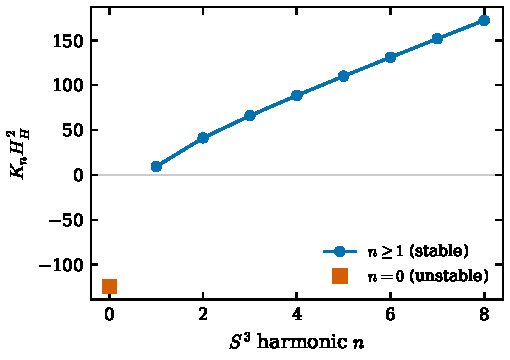
\includegraphics[width=\columnwidth]{figures/kernel}
\caption{Boundary fluctuation kernel $K_nH_H^2$ at $\mu^2=3$. The
homogeneous mode $n=0$ is the sole negative direction; all inhomogeneous
harmonics are Gaussian suppressed and the kernel grows approximately
linearly in $n$.}
\label{fig:kernel}
\end{figure}

The other sectors do not disturb this conclusion. For transverse-traceless
perturbations the gauge-fixed four-sphere operator is
$\mathcal{O}_{\rm TT}=-\Box_H+2H_H^2$; since the tensor-harmonic Laplacian
eigenvalues are $[L(L+3)-2]H_H^2$ for $L\ge2$, the physical tensor Hessian
has $\lambda_L^{\rm TT}=L(L+3)H_H^2>0$, so every physical tensor harmonic is
suppressed. Vector metric modes are pure gauge, and the scalar metric
constraints leave $\delta\phi$ as the only physical scalar because
$\dot\phi_H=0$ at the horizon. A gauge-fixed conformal determinant and its
contour are still required; positivity of the physical spectrum does not by
itself resolve the Euclidean conformal-factor problem, and we return to this
in Sec.~\ref{sec:discussion}.

We note one numerical point, since it is easy to encounter and silent when
it occurs. Imposing the regular behaviour literally as
$f_n(u_0)=u_0^{\,n}$ underflows the absolute tolerance of a standard
integrator for $n\gtrsim6$, after which the solution is numerical noise
rather than the regular mode. All results here normalize $f_n(u_0)=1$
instead, which is equivalent by linearity of Eq.~(\ref{eq:euclid}) and keeps
amplitudes of order unity throughout.

\section{The classicalizing contour and the admissible window}
\label{sec:thimble}

\subsection{The obstruction}
Because $K_0<0$, a real homogeneous boundary amplitude gives
\begin{equation}
\Psi(X_0)\propto\exp\!\left(+\frac{|K_0|X_0^2}{2\hbar}\right),
\end{equation}
an inverse Gaussian, which is not normalizable. The real Euclidean axis is
therefore inadmissible as the integration contour. The steepest-descent
direction of the fixed boundary kernel is instead $X_0=iY_0$, which restores
a normalizable Gaussian in $Y_0$ but at the cost of a purely imaginary
Euclidean displacement, with no evident connection to the real Lorentzian
rolling histories the saddle is supposed to initiate. Neither the real axis
nor the naive thimble is satisfactory, and the contour must be determined by
a physical requirement rather than by the Hessian alone.

\subsection{Selection by Lorentzian reality}
The requirement we impose is that the late-time growing branch be real, since
it is that branch which becomes the classical rolling history. Let $v=H_Ht$
after continuation through the equator and normalize the homogeneous
Euclidean mode to unity there, with logarithmic derivative
\begin{equation}
r_E=\frac{f_0'(\pi/2)}{f_0(\pi/2)} .
\end{equation}
For a complex equatorial amplitude $A$, continuation gives
$\delta\phi(0)=A$ and $\delta\phi_{,v}(0)=ir_EA$, and the Lorentzian mode
equation is
\begin{equation}
\delta\phi_{,vv}+3\tanh v\,\delta\phi_{,v}-\mu^2\,\delta\phi=0 .
\label{eq:lorentz}
\end{equation}
Writing the coefficient of the late growing solution as
$C_g=(c_1+ir_Ec_2)A$, where $c_1$ and $c_2$ are obtained by integrating
Eq.~(\ref{eq:lorentz}) from the initial data $(1,0)$ and $(0,1)$
respectively, reality of $C_g$ fixes the contour phase uniquely up to
orientation:
\begin{equation}
A=e^{i\theta}Y,\qquad
\theta=-\arg\!\left(c_1+ir_Ec_2\right),\qquad Y\in\mathbb{R}.
\label{eq:theta}
\end{equation}
Along this direction the real part of the exponent becomes
$\operatorname{Re}\ln\Psi=-\tfrac12|K_0|\cos(2\theta)\,Y^2/H_H^2$, so the
state is normalizable if and only if
\begin{equation}
\cos2\theta<0,
\qquad\text{i.e.}\qquad \theta>\frac{\pi}{4}.
\label{eq:normcond}
\end{equation}

\subsection{The admissible window}
Condition~(\ref{eq:normcond}) is not automatic. Evaluating $\theta(\mu^2)$
across the one-negative-mode range shows that it is violated at small
$\mu^2$ and satisfied at large $\mu^2$, with the crossing at
\begin{equation}
\boxed{\;\mu^2_{\rm crit}=\frac74\;}
\label{eq:crit}
\end{equation}
where $\theta=45^\circ$ exactly (Fig.~\ref{fig:window}). The threshold has a
structural origin. The exponents of Eq.~(\ref{eq:lorentz}) at late times are
$s$ and $-(3+s)$, where $s(s+3)=\mu^2$, that is
$s=\tfrac12[\sqrt{9+4\mu^2}-3]$; they differ by $2s+3$. At $\mu^2=7/4$ the
discriminant becomes a perfect square, $9+4\mu^2=16$, giving $s=1/2$ and
exponent difference exactly $4$. Over the open window $0<\mu^2<4$ the
difference $2s+3$ runs over $(3,5)$, so $\mu^2=7/4$ is the \emph{unique}
interior value at which the two exponents differ by an integer and the mode
equation degenerates. The loss of normalizability coincides with that
degeneracy.

The conclusion is that the one-negative-mode condition, which is the
standard admissibility criterion for a decay channel, is necessary but not
sufficient for a tachyonic horizon to support a normalizable classicalizing
state; the sharper requirement is Eq.~(\ref{eq:window}). Equivalently, in
terms of the growth rate, the unstable mode must satisfy $s>1/2$.
\begin{figure}
\centering
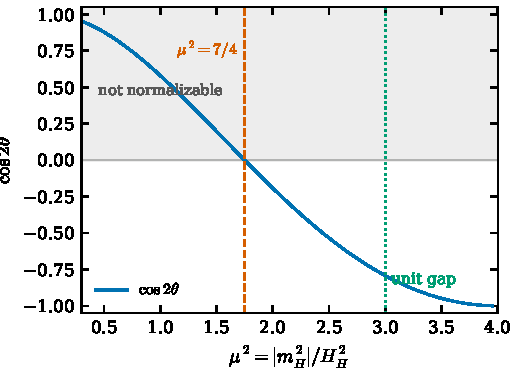
\includegraphics[width=\columnwidth]{figures/window}
\caption{Normalizability across the one-negative-mode window. The Born
measure on the classicalizing contour requires $\cos2\theta<0$, which fails
in the shaded region below $\mu^2=7/4$---exactly the point at which the two
Lorentzian exponents differ by an integer. The unit spectral gap $\mu^2=3$
lies inside the admissible range.}
\label{fig:window}
\end{figure}

\subsection{The state at the unit spectral gap}
At $\mu^2=d-1=3$ the construction gives $r_E=-6.27855862$,
$c_1=1.15455467$ and $c_2=0.54066085$, hence
\begin{equation}
\theta=71.215906^\circ,
\qquad
\cos2\theta=-0.79262829,
\end{equation}
so the contour is both classicalizing and convergent
(Fig.~\ref{fig:thimble}). With $K_0H_H^2=-123.9338$ the Born widths of the
equatorial amplitude and of the real growing coefficient are
\begin{equation}
\frac{\sigma_Y}{H_H}=0.07134,
\qquad
\frac{\sigma_{C_g}}{H_H}=0.25581,
\end{equation}
the latter following from
$\operatorname{Re}\ln\Psi(C_g)=-\tfrac12\kappa_CC_g^2/H_H^2$ with
$\kappa_C=7.64099$. It is this distribution, rather than a sharp initial
condition, that seeds the stochastic exit in Sec.~\ref{sec:exit}.
\begin{figure}
\centering
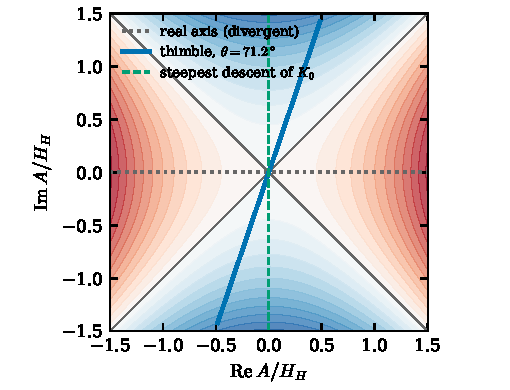
\includegraphics[width=\columnwidth]{figures/thimble}
\caption{The complex plane of the equatorial amplitude at $\mu^2=3$. Shading
gives the real part of the exponent, positive (divergent) along the real
axis. The steepest-descent direction of the boundary kernel is purely
imaginary; requiring the growing Lorentzian branch to be real instead selects
the contour at $\theta=71.216^\circ$, along which the measure is
normalizable.}
\label{fig:thimble}
\end{figure}

Two remarks place this result relative to existing criteria. First, the
selection here is made by reality of the growing branch rather than by a
WKB classicality condition of the type used in no-boundary analyses of
hilltop potentials \cite{HHH2008}, which for a scalar field requires
$m^2<(3H/2)^2$, i.e. $\mu^2<9/4$. The two criteria are distinct and act in
opposite directions: the present condition is a lower bound, $\mu^2>7/4$, and
a horizon at $\mu^2=3$ satisfies it while violating the WKB bound. There is
no contradiction, because the contours being tested are not the same;
the point is that classicalization must be established for the contour
actually used, and Eq.~(\ref{eq:theta}) does so by construction.

Second, the linear treatment is self-consistent in the region carrying
probability. For the worked example of the companion paper, the cubic term
of the local potential expansion produces a force smaller than the linear
force by a factor of $3\times10^{-6}$ at the drift threshold, and the
amplitude at which the cubic and linear forces become comparable lies at
$-\ln P\simeq2\times10^{10}$ in the Born measure. Nonlinear bending of the
contour is therefore negligible wherever the state has support.

\section{The lapse contour}
\label{sec:lapse}
Section~\ref{sec:thimble} fixed the contour over the scalar direction at
fixed geometry. The geometry must also be integrated, and the prescription
for doing so is not unique.

A strictly Dirichlet propagator from zero initial size, defined by a
positive-real Lorentzian lapse contour and deformed by Picard--Lefschetz
theory, is known to select tunneling-weight saddles and to generate
inverse-Gaussian perturbation spectra \cite{FLT2017,FLT2017b}. That
prescription is not admissible as the state of the present system, for the
same reason the real Euclidean axis was rejected above. A more suitable
formulation omits an artificial initial Gibbons--Hawking--York boundary term,
so that the variational problem fixes the initial momentum rather than the
initial size \cite{DiTucci2019}. Regular compact closure then requires the
Neumann condition
\begin{equation}
\left.\frac{\dot q}{2N}\right|_{t=0}=+i,
\qquad q\equiv a^2 .
\label{eq:neumann}
\end{equation}

At the frozen horizon the background minisuperspace problem is exactly the
closed de Sitter problem, because
$\nabla_\mu\phi_H=0$, $U_{,\phi}(\phi_H)=0$ and $U(\phi_H)=3\Mpl^2H_H^2$.
In the parametrization $ds^2=-(N^2/q)\,dt^2+q\,d\Omega_3^2$ with
Eq.~(\ref{eq:neumann}) and a final size $q(1)=q_1$, integrating out $q(t)$
gives the exact lapse action (in units $8\pi G=1$)
\begin{equation}
\frac{S_0(N)}{V_3}=H_H^4N^3+3iH_H^2N^2-3H_H^2q_1N-3iq_1 ,
\end{equation}
whose only saddles are
\begin{equation}
N_\pm=\pm\frac{\sqrt{H_H^2q_1-1}}{H_H^2}-\frac{i}{H_H^2} .
\label{eq:saddles}
\end{equation}
These are the expanding and contracting Hartle--Hawking saddles; the two
tunneling saddles carrying $+i/H_H^2$ are absent. Picard--Lefschetz flow
deforms the full real lapse line into $\mathbb{R}_N\sim\mathcal{J}_-+
\mathcal{J}_+$, so both retained saddles have nonvanishing intersection
number. The background contour question is thus settled exactly for this
saddle, rather than inferred from a local Hessian.

The scalar sector decouples from the lapse and metric perturbations at
quadratic order. Every mixed term in the Hessian carries either
$\nabla_\mu\phi_H$ or $U_{,\phi}(\phi_H)$, and both vanish at a frozen
horizon, so
\begin{equation}
\delta^2I_E=\delta^2I_{E,\rm grav}
+\frac12\int d^4x\sqrt{g_H}\,\delta\phi
\left(-\Box_H+U_{,\phi\phi}(\phi_H)\right)\delta\phi .
\end{equation}
Integrating the Gaussian lapse and metric fluctuations therefore cannot
alter the scalar kernel of Sec.~\ref{sec:kernel} or the contour phase of
Eq.~(\ref{eq:theta}) at this order. The leading scalar--metric coupling is
schematically $h(\delta\phi)^2$; eliminating $h$ feeds back into the scalar
effective action only at $O((\delta\phi)^4/\Mpl^2)$, which at the derived
exit width is suppressed by $(\sigma_{C_g}/\Mpl)^2\simeq2\times10^{-12}$ in
the worked example. Gravitational backreaction cannot overturn
normalizability.

Since the quadratic Hessian factorizes, the joint intersection number is the
product of the separate ones. The classicalizing scalar contour crosses the
real $C_g$ axis transversely once, giving $n_\phi=1$, and each retained
Neumann saddle has $n_N=1$, so
\begin{equation}
n_{(N,\phi)}=n_Nn_\phi=1
\end{equation}
for the expanding and contracting saddles alike. This integer is stable
under analytic deformation unless a critical-point collision, a singularity,
or a Stokes crossing intervenes; as noted in Sec.~\ref{sec:thimble}, the
nonlinear region is reached only at Born suppression
$-\ln P\sim10^{10}$, so the result holds throughout the region carrying
semiclassical probability. It does not exclude a global Stokes transition
driven by a distant saddle, and we return to that limitation in
Sec.~\ref{sec:discussion}.

\section{Discrete mode crossing on $S^3$}
\label{sec:shells}
Stochastic treatments of inflationary exit ordinarily model the
short-wavelength modes as a white-noise bath, on the grounds that modes cross
the Hubble radius continuously. That assumption fails immediately after a
finite-radius waist, because the spatial sections are $S^3$ and the harmonic
spectrum is discrete.

In closed slicing $a(v)=H_H^{-1}\cosh v$ and $aH_{\rm phys}=\sinh v$, so
harmonic $n$ crosses the Hubble scale when $\sinh v_n=\sqrt{n(n+2)}$. Since
$\cosh(\operatorname{arsinh}x)=\sqrt{1+x^2}$, the crossing times are exactly
\begin{equation}
\boxed{\;
v_n=\operatorname{arsinh}\sqrt{n(n+2)},
\qquad
N_n=\ln\frac{a(v_n)}{a(0)}=\ln(n+1).\;}
\label{eq:staircase}
\end{equation}
No inhomogeneous mode crosses during the first $\ln2=0.693$ scale-factor
e-folds, and the earliest crossings are individual shells rather than a
continuum. Equation~(\ref{eq:staircase}) is a property of closed de Sitter
slicing alone and involves no approximation.

The no-boundary state fixes the variance each shell contributes. With
$r_n=f_n'(\pi/2)/f_n(\pi/2)$ as in Sec.~\ref{sec:kernel} and $F_n(v)$ the
Lorentzian continuation normalized by $F_n(0)=1$, $F_{n,v}(0)=ir_n$, the
local variance added when shell $n$ enters the long-wavelength sector is
\begin{equation}
\frac{\Delta V_n}{H_H^2}=\frac{d_n\,|F_n(v_n)|^2}{4\pi^2 r_n},
\qquad d_n=(n+1)^2 .
\label{eq:shellvar}
\end{equation}
Table~\ref{tab:shells} gives the result. Defining an effective noise
amplitude by comparison with the continuum,
$Q^{\rm eff}_n=4\pi^2\Delta V_n/[H_H^2(N_n-N_{n-1})]$, the sequence
approaches the continuum horizon-crossing value $Q_\nu(1)=7.8686$ from above
and has converged to better than one percent by the eighth shell
(Fig.~\ref{fig:shells}). The agreement in the limit validates the
normalization of Eq.~(\ref{eq:shellvar}).
\begin{table}[htbp]\centering\small
\setlength{\tabcolsep}{4pt}
\begin{tabular}{r r r r r r}
\hline
$n$ & $N_n$ & $d_n$ & $|F_n(v_n)|$ & $\Delta V_n/H_H^2$ & $Q_n^{\rm eff}$ \\
\hline
1 & 0.69315 & 4 & 1.41992 & 0.427528 & 24.350 \\
2 & 1.09861 & 9 & 0.94168 & 0.096593 & 9.405 \\
3 & 1.38629 & 16 & 0.70426 & 0.060098 & 8.247 \\
4 & 1.60944 & 25 & 0.56259 & 0.044692 & 7.907 \\
5 & 1.79176 & 36 & 0.46843 & 0.035895 & 7.772 \\
6 & 1.94591 & 49 & 0.40131 & 0.030117 & 7.713 \\
7 & 2.07944 & 64 & 0.35103 & 0.025998 & 7.686 \\
8 & 2.19722 & 81 & 0.31195 & 0.022899 & 7.675 \\
\hline
\end{tabular}
\caption{Discrete $S^3$ shell crossings. Harmonic $n$ enters the long-wavelength sector at $N_n=\ln(n+1)$ exactly, injecting variance $\Delta V_n$. The effective noise amplitude $Q_n^{\rm eff}$ falls steeply and crosses the continuum value $Q_\nu(1)=7.8686$ between the fourth and fifth shells, undershooting it by $2.5\%$ at $n=8$; the first shell exceeds it by a factor of three.}
\label{tab:shells}
\end{table}

\begin{figure}
\centering
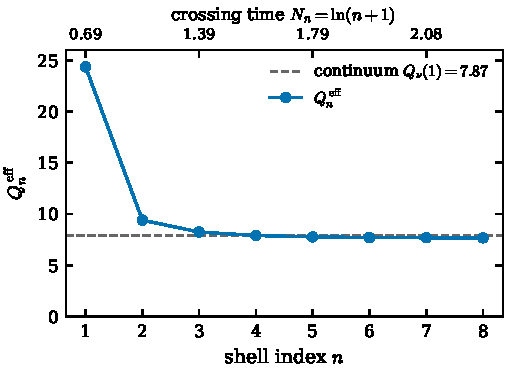
\includegraphics[width=\columnwidth]{figures/shells}
\caption{Effective noise amplitude injected by each $S^3$ shell, against
shell index and crossing time. The sequence converges rapidly to the
continuum value, but the first shell exceeds it by a factor of three,
precisely in the epoch where the exit occurs.}
\label{fig:shells}
\end{figure}

The first shell, however, has $Q_1^{\rm eff}=24.35$, three times the
continuum value. At Gaussian order the exact early influence functional is
therefore a discrete product, equivalently represented by jumps
\begin{equation}
X(N_n^+)=X(N_n^-)+\eta_n,
\qquad
\langle\eta_n\eta_m\rangle=\Delta V_n\,\delta_{nm},
\end{equation}
and noise kernel
\begin{equation}
\langle\xi(N)\xi(N')\rangle=\sum_{n\ge1}\Delta V_n\,
\delta(N-N_n)\,\delta(N'-N_n),
\end{equation}
rather than by a white-noise correlator. The continuum
kernel emerges only after many shells have crossed. Since the exit occurs
within the first few e-folds, this is exactly the regime in which the
continuum treatment is least reliable.

\section{Exit as a first-passage problem}
\label{sec:exit}
The coarse-grained unstable mode $X=\phi_H-\phi$ obeys
$dX=sX\,dN+\sigma_\epsilon\,dW_N$ with $s=\tfrac12[\sqrt{9+4\mu^2}-3]$. The
noise amplitude is not the familiar massless value. At a coarse-graining
boundary $k_c=\epsilon aH_H$ the exact de Sitter mode function gives
\begin{equation}
\sigma_\epsilon=\frac{H_H}{2\pi}\sqrt{Q_\nu(\epsilon)},
\qquad
Q_\nu(\epsilon)=\frac{\pi}{2}\epsilon^3\left|H^{(1)}_\nu(\epsilon)\right|^2,
\label{eq:kick}
\end{equation}
with $\nu=\sqrt{9/4+\mu^2}$. At $\mu^2=3$ this is $\nu=\sqrt{21}/2$ and
$\sqrt{Q_\nu(1)}=2.805$ at horizon crossing, so the massless expression
$H_H/2\pi$ underestimates the kick by nearly a factor of three. The
classicality boundary at which drift overtakes noise is
$X_c=\sigma_\epsilon/s$.

Two features distinguish the present treatment from a standard
Ornstein--Uhlenbeck escape. First, the initial condition is not sharp: the
process is seeded by the Born distribution of Sec.~\ref{sec:thimble}, with
$\sigma_{C_g}=0.25581H_H$, which is a substantial fraction of $X_c$ and
places a small part of the ensemble outside the classicality boundary from
the outset. Averaging the first-passage moments over that seed gives, at
$\epsilon=1$, a mean waiting time of $0.843$ e-folds with standard deviation
$0.821$, against $1.101\pm0.824$ for the sharp condition $X(0)=0$.

Second, and more significantly, Sec.~\ref{sec:shells} shows that the noise
during this epoch is discrete. Generating the process directly from the
no-boundary mode functions, with each shell added at its exact crossing time
$N_n=\ln(n+1)$ and with the homogeneous contribution sampled along the
classicalizing contour, produces an exit-time distribution whose quantiles
pile up at $\ln(n+1)$: the median history exits when the first inhomogeneous
shell crosses. This staircase is absent from the continuum treatment and is
a direct signature of the closed spatial sections.

Both results remain operational rather than predictive, for a reason that
should be stated plainly. The threshold $X_c$ is inherited from a continuum
drift-versus-noise criterion, and a physical decoherence or
branch-classicality condition must replace it before any duration is claimed
as a prediction. What is state-derived, and independent of that choice, is
the set of crossing times $N_n$ and the shell covariances $\Delta V_n$.

One consistency requirement deserves emphasis because it is easy to violate.
The classical e-fold count that follows the stochastic phase must be started
from the same threshold at which that phase ends. Using the tachyonic
boundary for the stochastic moments while retaining a classical count begun
at the massless boundary double-counts $\ln\sqrt{Q_\nu(1)}/s=1.303$ e-folds
of trajectory. With the thresholds matched, the worked example of the
companion paper gives a total duration of $74.40\pm0.82$ e-folds, which we
quote as a benchmark rather than a prediction.

\section{Observability of the staircase}
\label{sec:observability}
A discrete spectrum of crossing times is an arresting prediction, and it is
natural to ask whether it survives into the observable sky. It does not, and
the margin is very large.

After a patch classicalizes, the separate-universe map converts a growing
scalaron perturbation into the curvature perturbation,
$\zeta(\mathbf{x})=\delta N(\mathbf{x})$, so the lowest shells can in
principle create superhorizon differences between patches. Whether they are
observable depends on their present comoving scale. Ignoring an
order-unity ratio $H_n/H_*$, the shell-to-wavenumber map is
\begin{equation}
k_n\simeq k_*\exp\!\left[N_n-(N_{\rm tot}-N_*)\right],
\label{eq:kmap}
\end{equation}
where $N_*$ is the pivot's e-fold distance to the end of inflation and
$N_{\rm tot}$ the total duration. Both are model-dependent, and we take them
from the worked example of the companion paper: $N_*=50.585$ and
$N_{\rm tot}=74.403$ with $k_*=0.05\Mpc$. The first shell then lies at
\begin{equation}
k_{n=1}\simeq4.5\times10^{-12}\Mpc,
\qquad
\ell_{n=1}\sim k_{n=1}\chi_*\simeq6\times10^{-8},
\end{equation}
which is smaller than the present horizon scale by some eight orders of
magnitude. At the wall-induced feature of the companion paper,
$k\simeq9.2\times10^{-5}\Mpc$, the corresponding shell index and spacing are
\begin{equation}
n\simeq4\times10^{7},
\qquad
\Delta\ln k\simeq n^{-1}\simeq2\times10^{-8},
\end{equation}
so the closed-shell spectrum is indistinguishable from a continuum
throughout the observable range, to one part in $10^{7}$. We conclude that
the $\ln(n+1)$ staircase produces no observable signature in the cosmic
microwave background.

This is a negative result, and it should be read as delimiting the reach of
the analysis rather than diminishing it. The discreteness established in
Sec.~\ref{sec:shells} is a property of the initial quantum state, exact and
state-derived, but the observable universe samples only the deep continuum
tail of the sequence. Any observable low-multipole signature of such a model
must therefore arise from the subsequent inflationary dynamics---in the
worked example, the wall-induced primordial transfer analyzed in the
companion paper \cite{PandevI}---and not from the discreteness of the
beginning.

\section{Discussion}
\label{sec:discussion}
The analysis establishes a definite quantum state for a tachyonic $f(R)$
horizon within a well-specified domain, and it is worth separating that
domain from what lies outside it.

Three limitations are structural rather than technical. First, the
intersection-number result of Sec.~\ref{sec:lapse} is established throughout
the region carrying semiclassical probability, using the stability of the
integer under analytic deformation; it does not exclude a global Stokes
transition induced by a distant saddle, which would require a full
upward-flow computation over the infinite-dimensional cycle. Second, the
positivity of the physical scalar and tensor spectra does not by itself
resolve the Euclidean conformal-factor problem: a gauge-fixed conformal
determinant and its own contour prescription are still required, and until
they are supplied the state is defined on the physical sector rather than on
the full configuration space. Third, the duration quoted in
Sec.~\ref{sec:exit} rests on a threshold borrowed from a continuum
drift criterion. A decoherence or branch-classicality condition derived from
the reduced density matrix must replace it, and doing so would also
eliminate the residual dependence on the coarse-graining parameter
$\epsilon$, which at present is mild but not absent.

Set against these, the window $7/4<\mu^2<4$ appears robust. It follows from
the reality requirement and the normalizability condition alone, both of
which are properties of the quadratic theory, and its lower edge coincides
with an exact degeneracy of the mode equation rather than with a numerical
accident. The result constrains model building directly: a construction
that places a tachyonic horizon at $\mu^2\le7/4$ does not admit a
normalizable classicalizing state of the kind derived here, whatever
curvature function produces the horizon. That the unit spectral gap
$\mu^2=d-1=3$ falls inside the window with margin is a nontrivial
consistency check on the bootstrap of the companion paper, though it is not
a derivation of that condition.

\section{Conclusions}
\label{sec:conclusions}
The principal results of this work are the following.

\begin{enumerate}
\item For a tachyonic horizon in metric $f(R)$ gravity, requiring the growing
Lorentzian branch to be real selects the integration contour over the
unstable direction uniquely, at an angle $\theta(\mu^2)$ given by
Eq.~(\ref{eq:theta}). The Born measure along that contour is normalizable
only for $7/4<\mu^2<4$. The one-negative-mode condition $0<\mu^2<4$, which is
the standard admissibility criterion for a decay channel, is therefore
necessary but not sufficient.

\item The threshold is exact and structural. At $\mu^2=7/4$ the growth
exponent is $s=1/2$, so the Lorentzian exponents $s$ and $-(3+s)$ differ by
exactly four; this is the unique point interior to the one-negative-mode
window at which they differ by an integer and the mode equation degenerates.

\item At the unit spectral gap $\mu^2=3$ the boundary kernel has the Morse
structure required of a decay channel: the homogeneous mode is the sole
negative direction, and all inhomogeneous scalar and physical tensor
harmonics are Gaussian suppressed. The classicalizing contour lies at
$\theta=71.216^\circ$, with Born widths $\sigma_Y=0.0713H_H$ and
$\sigma_{C_g}=0.2558H_H$.

\item Under a Neumann regularity condition the background lapse integral can
be performed exactly. It retains the two Hartle--Hawking saddles with
nonvanishing intersection numbers and eliminates the tunneling pair. Scalar
and metric perturbations decouple at quadratic order, so the joint
intersection number is unity throughout the region carrying semiclassical
probability, and gravitational backreaction is suppressed by
$O(10^{-12})$ at the derived exit width.

\item On $S^3$ sections the early noise is discrete rather than white:
harmonic $n$ enters the long-wavelength sector at $N_n=\ln(n+1)$ exactly, no
inhomogeneous mode crosses during the first $\ln2$ e-folds, and the first
shell injects three times the continuum variance. The exit is consequently a
discrete first-passage process whose exit-time quantiles pile up at
$\ln(n+1)$. The findings indicate that continuum stochastic treatments are
not reliable in the epoch immediately following a finite-radius waist.

\item The staircase is nevertheless unobservable. In the worked example the
first shell maps to $k\simeq4.5\times10^{-12}\Mpc$, and at observable scales
the shell spacing is $\Delta\ln k\simeq2\times10^{-8}$. The discreteness is a
property of the initial state and not of the sky.
\end{enumerate}

Two developments would materially extend these conclusions: a decoherence
criterion derived from the reduced density matrix, which would convert the
duration from a benchmark into a prediction; and a treatment of the
conformal-factor contour, which would extend the state from the physical
sector to the full configuration space.

\section*{Declarations}
\paragraph{Funding.} No funding was received for this work.
\paragraph{Conflict of interest.} The author declares no competing
interests.
\paragraph{Use of AI tools.} The author used Anthropic's Claude to assist
with the code, figures, and text; the author verified all results and takes
full responsibility for the content.
\paragraph{Data and code availability.} All numerical results in this paper
regenerate from the released code, archived at
\href{https://doi.org/10.5281/zenodo.21829379}{doi:10.5281/zenodo.21829379}
and developed at \url{https://github.com/spsingularity/frozen-horizon}; every table and figure in this manuscript is a build artifact
of that pipeline.

\bibliographystyle{spphys}
\bibliography{refs}

\end{document}
